
\subsection{Caso: \( D = 0.1 \)}

% T = 0
\subsubsection{Análise para o caso: \( D = 0.1 \) e \( t = 0 \)}

A Figura \ref{fig:advec_diffus_0.1_t0} mostra a distribuição da concentração de soluto no tempo inicial para um coeficiente de difusão \( D = 0.1 \). Como observado, a solução de advecção-difusão mostra uma suavização inicial e um alargamento da distribuição da concentração em comparação com a advecção pura, que mantém a forma original da distribuição de concentração estabelecida pela condição inicial. Este efeito é típico de processos difusivos, onde a concentração tende a se espalhar para fora de sua posição inicial mais rapidamente.

\begin{figure}[H]
    \centering
    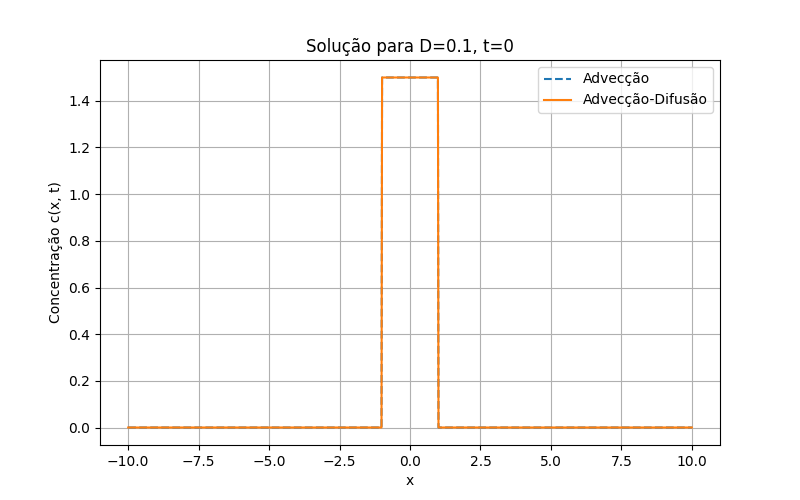
\includegraphics[width=0.7\textwidth]{code/plot/Advec_Difus_t0_D0.1.png}
    \caption{Comparação das soluções de advecção e advecção-difusão para \( D = 0.1 \) no tempo \( t = 0 \). A linha tracejada representa a advecção pura, enquanto a linha contínua indica a advecção-difusão.}
    \label{fig:advec_diffus_0.1_t0}
\end{figure}


\begin{table}[H]
    \centering
    \caption{Valores numéricos da concentração para \( D = 0.1 \) e \( t = 0 \)}
    \begin{tabular}{ccc}
\toprule
x & Advecção & Advecção-Difusão \\
\midrule
-2.250000 & 0.000000 & 0.000000 \\
-1.690000 & 0.000000 & 0.000000 \\
-1.140000 & 0.000000 & 0.000000 \\
-0.580000 & 1.500000 & 1.500000 \\
-0.030000 & 1.500000 & 1.500000 \\
0.530000 & 1.500000 & 1.500000 \\
1.080000 & 0.000000 & 0.000000 \\
1.640000 & 0.000000 & 0.000000 \\
2.190000 & 0.000000 & 0.000000 \\
2.750000 & 0.000000 & 0.000000 \\
\bottomrule
\end{tabular}

\end{table}


% T = 1
\subsubsection{Análise para o caso: \( D = 0.1 \) e \( t = 1 \)}

A Figura \ref{fig:advec_diffus_0.1_t1} mostra a distribuição da concentração de soluto no tempo \( t = 1 \) para um coeficiente de difusão \( D = 0.1 \). A advecção pura mantém a forma original retangular, simplesmente deslocada, enquanto a advecção-difusão revela uma significativa suavização e espalhamento da concentração, característico de um processo onde a difusão tem um papel importante.

\begin{figure}[H]
    \centering
    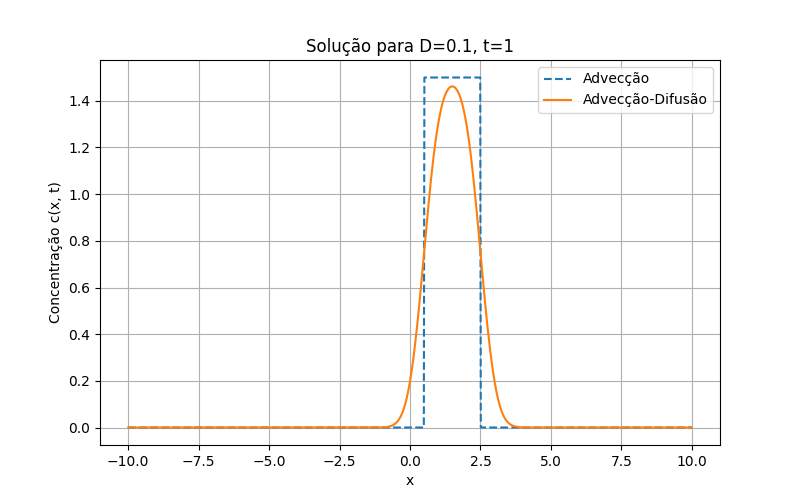
\includegraphics[width=0.7\textwidth]{code/plot/Advec_Difus_t1_D0.1.png}
    \caption{Comparação das soluções de advecção e advecção-difusão para \( D = 0.1 \) no tempo \( t = 1 \). A linha tracejada representa a advecção pura, enquanto a linha contínua indica a advecção-difusão.}
    \label{fig:advec_diffus_0.1_t1}
\end{figure}

\begin{table}[H]
    \centering
    \caption{Valores numéricos da concentração para \( D = 0.1 \) e \( t = 1 \)}
    \begin{tabular}{ccc}
\toprule
x & Advecção & Advecção-Difusão \\
\midrule
-0.750000 & 0.000000 & 0.003891 \\
-0.190000 & 0.000000 & 0.090349 \\
0.360000 & 0.000000 & 0.567097 \\
0.920000 & 1.500000 & 1.236080 \\
1.470000 & 1.500000 & 1.461555 \\
2.030000 & 1.500000 & 1.281271 \\
2.580000 & 0.000000 & 0.639132 \\
3.140000 & 0.000000 & 0.114840 \\
3.690000 & 0.000000 & 0.005674 \\
4.250000 & 0.000000 & 0.000068 \\
\bottomrule
\end{tabular}

\end{table}


% T = 2
\subsubsection{Análise para o caso: \( D = 0.1 \) e \( t = 2 \)}

A Figura \ref{fig:advec_diffus_0.1_t2} mostra a distribuição da concentração de soluto no tempo \( t = 2 \) para um coeficiente de difusão \( D = 0.1 \). A diferença entre a advecção pura e a advecção-difusão torna-se ainda mais evidente, com a difusão claramente aumentando o espalhamento do soluto além da simples deslocação causada pela advecção.

\begin{figure}[H]
    \centering
    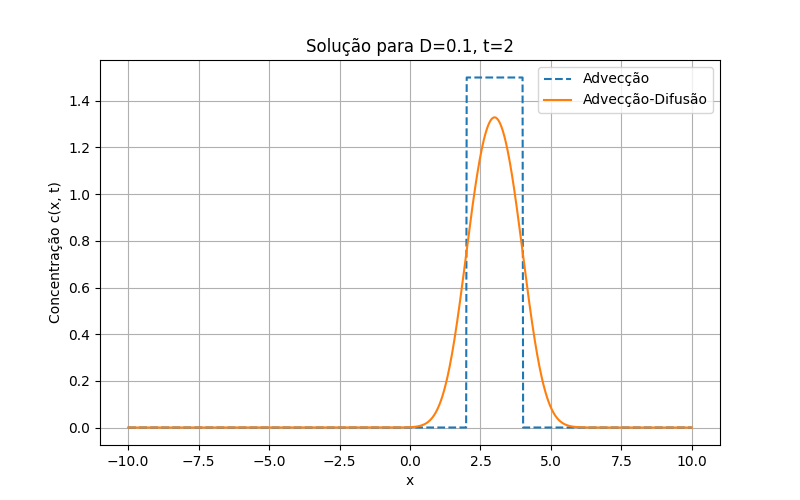
\includegraphics[width=0.7\textwidth]{code/plot/Advec_Difus_t2_D0.1.png}
    \caption{Comparação das soluções de advecção e advecção-difusão para \( D = 0.1 \) no tempo \( t = 2 \). A linha tracejada representa a advecção pura, enquanto a linha contínua indica a advecção-difusão, mostrando maior dispersão.}
    \label{fig:advec_diffus_0.1_t2}
\end{figure}

\begin{table}[H]
    \centering
    \caption{Valores numéricos da concentração para \( D = 0.1 \) e \( t = 2 \)}
    \begin{tabular}{ccc}
\toprule
x & Advecção & Advecção-Difusão \\
\midrule
0.750000 & 0.000000 & 0.036080 \\
1.310000 & 0.000000 & 0.204134 \\
1.860000 & 0.000000 & 0.619096 \\
2.420000 & 1.500000 & 1.108262 \\
2.970000 & 1.500000 & 1.328708 \\
3.530000 & 1.500000 & 1.146762 \\
4.080000 & 0.000000 & 0.670639 \\
4.640000 & 0.000000 & 0.234287 \\
5.190000 & 0.000000 & 0.044211 \\
5.750000 & 0.000000 & 0.004243 \\
\bottomrule
\end{tabular}

\end{table}

% T = 3
\subsubsection{Análise para o caso: \( D = 0.1 \) e \( t = 3 \)}

A Figura \ref{fig:advec_diffus_0.1_t3} mostra a distribuição da concentração de soluto no tempo \( t = 3 \) para um coeficiente de difusão \( D = 0.1 \). Observa-se que a diferença entre a advecção pura e a advecção-difusão é acentuada, com a difusão produzindo um perfil de concentração significativamente mais suavizado e espalhado.

\begin{figure}[H]
    \centering
    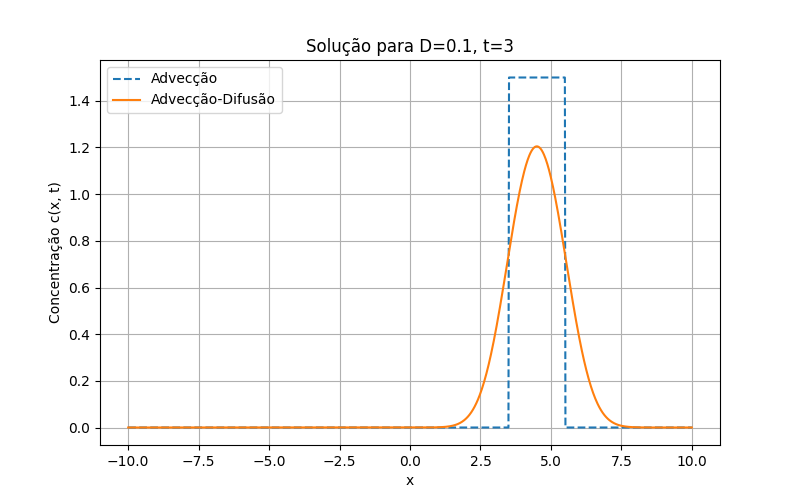
\includegraphics[width=0.7\textwidth]{code/plot/Advec_Difus_t3_D0.1.png}
    \caption{Comparação das soluções de advecção e advecção-difusão para \( D = 0.1 \) no tempo \( t = 3 \). A linha tracejada representa a advecção pura, enquanto a linha contínua indica a advecção-difusão, destacando o aumento da dispersão.}
    \label{fig:advec_diffus_0.1_t3}
\end{figure}

\begin{table}[H]
    \centering
    \caption{Valores numéricos da concentração para \( D = 0.1 \) e \( t = 3 \)}
    \begin{tabular}{ccc}
\toprule
x & Advecção & Advecção-Difusão \\
\midrule
2.250000 & 0.000000 & 0.079917 \\
2.810000 & 0.000000 & 0.277102 \\
3.360000 & 0.000000 & 0.638956 \\
3.920000 & 1.500000 & 1.026313 \\
4.470000 & 1.500000 & 1.204510 \\
5.030000 & 1.500000 & 1.056996 \\
5.580000 & 0.000000 & 0.680379 \\
6.140000 & 0.000000 & 0.306620 \\
6.690000 & 0.000000 & 0.092273 \\
7.250000 & 0.000000 & 0.017900 \\
\bottomrule
\end{tabular}

\end{table}


% T = 4
\subsubsection{Análise para o caso: \( D = 0.1 \) e \( t = 4 \)}

A Figura \ref{fig:advec_diffus_0.1_t4} mostra a distribuição da concentração de soluto no tempo \( t = 4 \) para um coeficiente de difusão \( D = 0.1 \). O perfil de advecção-difusão agora exibe um pico ainda mais concentrado e caudas mais extensas, evidenciando a influência crescente da difusão na forma da distribuição da concentração.

\begin{figure}[H]
    \centering
    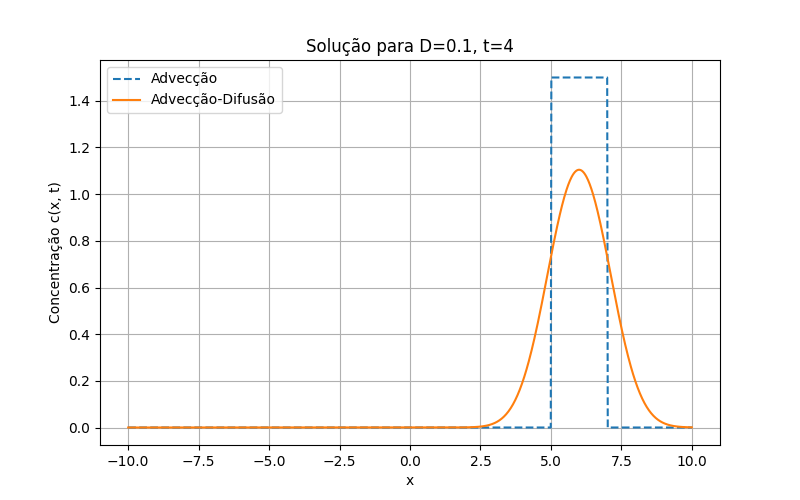
\includegraphics[width=0.7\textwidth]{code/plot/Advec_Difus_t4_D0.1.png}
    \caption{Comparação das soluções de advecção e advecção-difusão para \( D = 0.1 \) no tempo \( t = 4 \). A linha tracejada representa a advecção pura, enquanto a linha contínua indica a advecção-difusão, mostrando um aumento na dispersão e na concentração do pico.}
    \label{fig:advec_diffus_0.1_t4}
\end{figure}

\begin{table}[H]
    \centering
    \caption{Valores numéricos da concentração para \( D = 0.1 \) e \( t = 4 \)}
    \begin{tabular}{ccc}
\toprule
x & Advecção & Advecção-Difusão \\
\midrule
3.750000 & 0.000000 & 0.121478 \\
4.310000 & 0.000000 & 0.326186 \\
4.860000 & 0.000000 & 0.644859 \\
5.420000 & 1.500000 & 0.961489 \\
5.970000 & 1.500000 & 1.104326 \\
6.530000 & 1.500000 & 0.986143 \\
7.080000 & 0.000000 & 0.679442 \\
7.640000 & 0.000000 & 0.353901 \\
8.190000 & 0.000000 & 0.136036 \\
8.750000 & 0.000000 & 0.037779 \\
\bottomrule
\end{tabular}

\end{table}


% T = 5
\subsubsection{Análise para o caso: \( D = 0.1 \) e \( t = 5 \)}

A Figura \ref{fig:advec_diffus_0.1_t5} mostra a distribuição da concentração de soluto no tempo \( t = 5 \) para um coeficiente de difusão \( D = 0.1 \). A diferença entre a advecção pura e a advecção-difusão é ainda mais acentuada, com a difusão resultando em uma dispersão substancial da concentração de soluto, suavizando e alargando significativamente o pico da distribuição.

\begin{figure}[H]
    \centering
    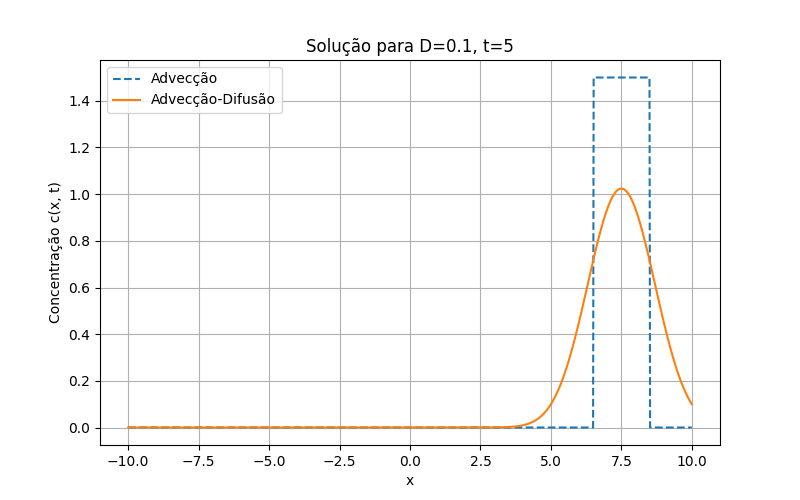
\includegraphics[width=0.7\textwidth]{code/plot/Advec_Difus_t5_D0.1.png}
    \caption{Comparação das soluções de advecção e advecção-difusão para \( D = 0.1 \) no tempo \( t = 5 \). A linha tracejada representa a advecção pura, enquanto a linha contínua indica a advecção-difusão, destacando uma dispersão ainda maior.}
    \label{fig:advec_diffus_0.1_t5}
\end{figure}

\begin{table}[H]
    \centering
    \caption{Valores numéricos da concentração para \( D = 0.1 \) e \( t = 5 \)}
    \begin{tabular}{ccc}
\toprule
x & Advecção & Advecção-Difusão \\
\midrule
5.250000 & 0.000000 & 0.157609 \\
5.810000 & 0.000000 & 0.360265 \\
6.360000 & 0.000000 & 0.642820 \\
6.920000 & 1.500000 & 0.907299 \\
7.470000 & 1.500000 & 1.023754 \\
8.030000 & 1.500000 & 0.927498 \\
8.580000 & 0.000000 & 0.672274 \\
9.140000 & 0.000000 & 0.385933 \\
9.690000 & 0.000000 & 0.173177 \\
10.250000 & 0.000000 & 0.059956 \\
\bottomrule
\end{tabular}

\end{table}


% Conclusão do Caso
\subsection{Conclusão do Caso: \( D = 0.1 \)}
Ao longo do intervalo observado de \( t = 0 \) a \( t = 5 \), as soluções numéricas da equação de advecção-difusão com coeficiente de difusão \( D = 0.1 \) revelaram mudanças significativas na distribuição da concentração de soluto. Inicialmente, advecção pura e advecção-difusão partem de um perfil retangular idêntico, mas logo divergem conforme a difusão começa a suavizar e alargar o perfil de concentração. Com o tempo, esse efeito se intensifica, resultando em uma diferença marcante por \( t = 5 \), onde a distribuição influenciada pela difusão mostra um pico mais pronunciado e extenso. Esta evolução destaca como mesmo uma moderada difusão de \( D = 0.1 \) pode transformar significativamente a dinâmica do transporte de solutos, enfatizando a importância de considerar a difusão em aplicações práticas onde a dispersão uniforme é crucial.